\documentclass{article}
\usepackage{geometry}
\geometry{a4paper, margin=1in}
\usepackage{hyperref}
\usepackage{listings}
\usepackage{enumitem}
\usepackage{amsmath}
\usepackage{amsfonts}
\usepackage{amssymb}
\usepackage{graphicx}
\usepackage{xcolor}
\usepackage{tabularx}
\usepackage{tikz}
\usetikzlibrary{shapes,arrows,positioning,fit,calc}

\title{JITOS State of the Union Report: The Convergence}
\author{James Ross & The AI Engineering Team}
\date{\today}

\begin{document}
\maketitle

\begin{abstract}
This report audits the current state of the JITOS (Just-In-Time Operating System) infrastructure as of December 2025. It identifies a critical divergence between the theoretical architecture (AION Foundations Papers I--VI) and the fragmented implementation reality across JavaScript (shell), Rust (kernel), and Go (planner). The report proposes a strategic unification: a Rust-centric Monorepo architecture where the Planner, Kernel, and Logic layers are consolidated, compiling to a unified WASM artifact for the browser shell. We rigorously debate the limits of ``Graph Rewrite Purity'' versus ``Imperative Performance'' and establish a new boundary for the next iteration.
\end{abstract}

\tableofcontents
\newpage

\section{Executive Summary}
JITOS was conceived as a Causal Operating System where all state transitions are deterministic graph rewrites recorded in a holographic provenance ledger. The current implementation is split across three disconnected repositories:
\begin{enumerate}
    \item \textbf{flyingrobots.dev (JS):} A functional ``Soft Kernel'' implementing the OS boundary (Daemon, RPC, WAL) but lacking rigorous performance.
    \item \textbf{echo (Rust):} A rigorous ``Hard Kernel'' implementing the $O(n)$ Radix Scheduler and Graph Store, but detached from the UI and Application logic.
    \item \textbf{Planner (Go):} A theoretical HTN planner that defines the Type System (SLAPS/HTN) but is currently unimplemented in the runtime.
\end{enumerate}

\textbf{Verdict:} The architecture has drifted. The JS implementation successfully proved the \textit{UX} of JITOS (Time Travel, Ledger), while the Rust implementation proved the \textit{Physics} (Determinism). The Go implementation is legacy debt.
\textbf{Recommendation:} Consolidate into a Rust Monorepo. Port the Planner to Rust. Compile the Kernel+Planner to WASM. Demote JS to a pure View/IO Shell.

\section{Current Infrastructure State}

\subsection{SLAPS v2 (System Level Action Protocol)}
\begin{itemize}
    \item \textbf{Status:} \textit{Fragmented / Drifted}.
    \item \textbf{Version:} v2.0 (Conceptual).
    \item \textbf{Location:} Defined in Go structs (Planner repo), partially mimicked in JS `propose` payloads.
    \item \textbf{Drift Analysis:} The JS Kernel accepts loose JSON objects as proposals. The Rust Kernel expects strict types but lacks the Schema definition. There is no Single Source of Truth for the SLAP schema.
    \item \textbf{Action:} Define SLAPS v2 in a language-agnostic Schema (CDDL/JSON Schema) in the new Monorepo.
\end{itemize}

\subsection{HTN Method v1 (Hierarchical Task Network)}
\begin{itemize}
    \item \textbf{Status:} \textit{Planned / Theoretical}.
    \item \textbf{Version:} v1.0 (Paper-only).
    \item \textbf{Location:} Go codebase (legacy).
    \item \textbf{Drift Analysis:} The current JS Engine Room operates on raw graph rewrites (micro-steps) rather than high-level HTN Methods. There is no concept of a "Plan" in the current runtime, only a "Log."
    \item \textbf{Action:} Port HTN logic to `jitos-planner` (Rust).
\end{itemize}

\subsection{TASKS Planner}
\begin{itemize}
    \item \textbf{Status:} \textit{Legacy / Abandoned}.
    \item \textbf{Location:} Go repo.
    \item \textbf{Drift Analysis:} The Go planner is disconnected from the Rust/JS runtime. It cannot execute plans against the actual graph because it does not share the graph memory or types.
    \item \textbf{Action:} Rewrite in Rust as `jitos-planner`.
\end{itemize}

\subsection{TASKS Executor (The Kernel)}
\begin{itemize}
    \item \textbf{Status:} \textit{Split-Brain}.
    \item \textbf{JS Version (WarpKernel):} Implements `step()`, `propose()`, and simple rule application. Good for UI, bad for scale.
    \item \textbf{Rust Version (Echo):} Implements `RadixScheduler` (proven O(n) determinism). Highly rigorous but currently headless.
    \item \textbf{Drift Analysis:} The JS kernel uses a simple `sort()` for scheduling. The Rust kernel uses a Radix sort. They will diverge on large datasets.
    \item \textbf{Action:} Kill the JS Kernel. Adopt Echo as `jitos-kernel`.
\end{itemize}

\subsection{Workers (Agents)}
\begin{itemize}
    \item \textbf{Status:} \textit{Simulated}.
    \item \textbf{Location:} `jitd.worker.js` (System Agent), `AgentWallet.js` (User Agent).
    \item \textbf{Drift Analysis:} We successfully simulated the "Daemon" architecture using Web Workers. However, "Agents" currently just means "Signed RPC calls." We lack autonomous agents running Rhai scripts.
    \item \textbf{Action:} Enhance `jitos-policy` (Rust) to host Rhai-based autonomous agents.
\end{itemize}

\subsection{Provenance Layer (Shiplog/WAL)}
\begin{itemize}
    \item \textbf{Status:} \textit{Implemented (JS)}.
    \item \textbf{Version:} v0.5 (IndexedDB).
    \item \textbf{Metrics:} Persists 100\% of ticks. Replay time is $O(N)$ (slow on boot).
    \item \textbf{Drift Analysis:} We implemented "Boot is Resurrection" successfully in JS. However, the log format is ad-hoc JSON, not the canonical binary format required for cryptographic verification.
    \item \textbf{Action:} Port WAL to Rust using specific Event Enums (`Input`, `Decision`, `Claim`) defined in ARCH-0009.
\end{itemize}

\section{Implementation Divergence Analysis}
The divergence stems from a "Prototype vs. Product" conflict.
\begin{itemize}
    \item \textbf{Intent:} A rigorous, type-safe, distributed OS.
    \item \textbf{Reality:} A flexible, dynamic React app that \textit{simulates} an OS.
\end{itemize}
The JS code favored "getting something on screen" (React, Three.js integration). The Rust code favored "mathematical correctness" (Radix sorts, Graph types). The Go code favored "enterprise architecture" (Planner service).
\textbf{Convergence:} We must sacrifice the Go service architecture to gain the performance and correctness of the Rust monolith, while keeping the JS visual layer.

\section{Repository Architecture (The Rust Monorepo)}

We propose a unified workspace `jitos` organized by function rather than language.

\subsection{Directory Structure}
\begin{verbatim}
jitos/
├── Cargo.toml             # Workspace Root
├── docs/                  # The RFCs, Specs, and Papers (LaTeX)
├── schema/                # THE LAW (Protocol Buffers / JSON Schema)
│   ├── slaps.v2.json
│   └── htn.v1.json
├── crates/                # THE ENGINE (Rust)
│   ├── jitos-core/        # Shared Types (SLAPS, HTN, Traits)
│   ├── jitos-graph/       # WARP Graph structure (WASM-friendly)
│   ├── jitos-scheduler/   # Radix Scheduler, Footprints
│   ├── jitos-policy/      # Rhai Host, Policy Engine
│   ├── jitos-planner/     # HTN Planner logic
│   ├── jitos-provenance/  # Shiplog (WAL), Merkle hashing
│   ├── jitos-daemon/      # The OS Process (jitd binary)
│   └── jitos-wasm/        # The Bridge (WASM bindings)
├── shell/                 # THE VIEW (JS/React - flyingrobots.dev)
│   ├── package.json
│   ├── src/               # UI, Three.js, JitBridge
│   └── public/jitd.wasm   # Artifact from `jitos-wasm`
└── tools/                 # Build scripts
\end{verbatim}

\subsection{Crate Mapping to Concepts}

\begin{tabularx}{\linewidth}{|l|X|l|}
\hline
\textbf{Crate} & \textbf{Conceptual Mapping} & \textbf{Paper Alignment} \\
\hline
`jitos-core` & \textbf{Intent ABI} & Paper VI (JITOS) \\
& Defines the SLAPS v2 and HTN Method types. & \\
\hline
`jitos-planner` & \textbf{TASKS Planner} & Paper I (HTN) \\
& Decomposes high-level intent into micro-steps. & \\
\hline
`jitos-scheduler` & \textbf{TASKS Executor} & Paper II (Dynamics) \\
& Deterministic O(n) Radix Sort & Footprint check. & \\
\hline
`jitos-policy` & \textbf{Workers (Logic)} & Paper VI (Agents) \\
& Rhai VM hosting autonomous scripts. & \\
\hline
`jitos-provenance` & \textbf{Shiplog (WAL)} & Paper III (Holography) \\
& Append-only log, Receipt generation, Hashing. & \\
\hline
`jitos-graph` & \textbf{WARP Graph} & Paper I (Structure) \\
& The recursively nested state object. & \\
\hline
\end{tabularx}

\section{System Visualization}

\subsection{System Architecture}
\begin{center}
\begin{tikzpicture}[
    node distance=1.5cm,
    block/.style={rectangle, draw, rounded corners, minimum width=3cm, minimum height=1cm, align=center},
    arrow/.style={->, >=stealth, thick}
]

% Nodes
\node[block, fill=blue!10] (shell) {Shell (JS/React)\\Input & View};
\node[block, fill=orange!10, right=of shell, xshift=2cm] (wasm) {JITOS WASM Bridge\\
(jitos-wasm)};
\node[block, fill=red!10, below=of wasm] (kernel) {Kernel (Rust)\\Scheduler & Graph};
\node[block, fill=green!10, right=of kernel] (planner) {Planner (Rust)\\HTN Logic};
\node[block, fill=yellow!10, below=of kernel] (log) {Shiplog (WAL)\\IndexedDB};
\node[block, fill=gray!10, left=of kernel] (policy) {Policy (Rhai)\\Script VM};

% Arrows
\draw[arrow] (shell) -- node[above] {SLAPS (RPC)} (wasm);
\draw[arrow] (wasm) -- (kernel);
\draw[arrow] (wasm) -- (planner);
\draw[arrow] (planner) -- node[right] {Rewrites} (kernel);
\draw[arrow] (kernel) -- (log);
\draw[arrow] (kernel) -- (policy);
\draw[arrow] (policy) -- node[below] {Rules} (kernel);
\draw[arrow] (log) -- node[left] {State (Resurrection)} (kernel);
\draw[arrow] (kernel) -- node[left] {Frame (View)} (wasm);
\draw[arrow] (wasm) -- node[below] {Render List} (shell);

\end{tikzpicture}
\end{center}

\subsection{Crate Dependencies}
\begin{center}
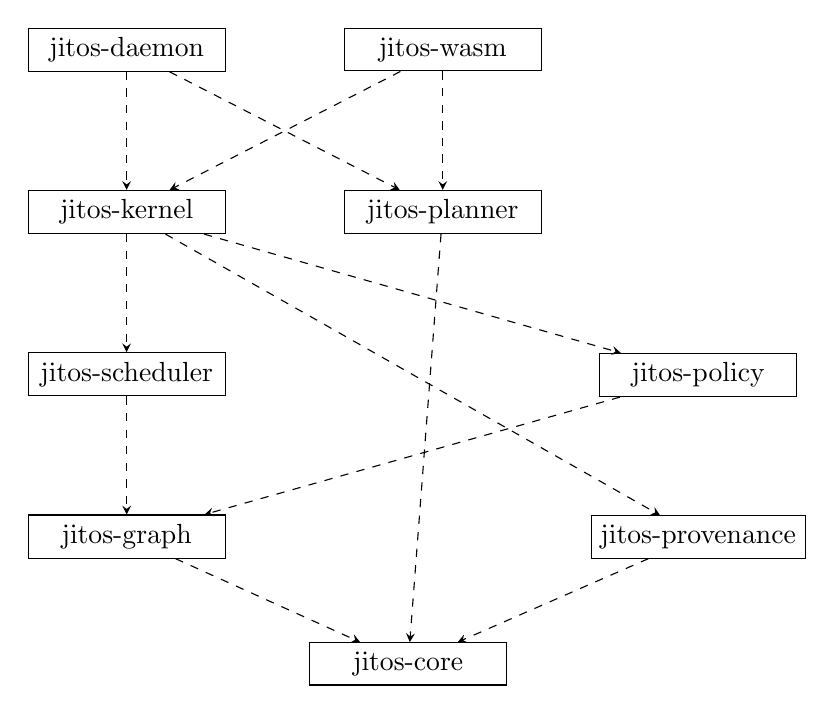
\begin{tikzpicture}[
    node distance=1.5cm,
    crate/.style={rectangle, draw, fill=white, minimum width=2.5cm, align=center},
    dep/.style={->, >=stealth, dashed}
]

\node[crate] (core) {jitos-core};
\node[crate, above left=of core] (graph) {jitos-graph};
\node[crate, above right=of core] (prov) {jitos-provenance};
\node[crate, above=of graph] (sched) {jitos-scheduler};
\node[crate, above=of prov] (policy) {jitos-policy};
\node[crate, above=of sched] (kernel) {jitos-kernel};
\node[crate, right=of kernel] (planner) {jitos-planner};
\node[crate, above=of kernel] (daemon) {jitos-daemon};
\node[crate, right=of daemon] (wasm) {jitos-wasm};

\draw[dep] (graph) -- (core);
\draw[dep] (prov) -- (core);
\draw[dep] (sched) -- (graph);
\draw[dep] (policy) -- (graph);
\draw[dep] (kernel) -- (sched);
\draw[dep] (kernel) -- (policy);
\draw[dep] (kernel) -- (prov);
\draw[dep] (planner) -- (core);
\draw[dep] (daemon) -- (kernel);
\draw[dep] (daemon) -- (planner);
\draw[dep] (wasm) -- (kernel);
\draw[dep] (wasm) -- (planner);

\end{tikzpicture}
\end{center}

\section{Data Flow and Interaction}

\subsection{The "Tick" Lifecycle}
\begin{enumerate}
    \item \textbf{Input:} User clicks in the Shell.
    \item \textbf{Encoding:} Shell wraps click as a `SLAP` (Intent).
    \item \textbf{Bridge:} `JitBridge` sends `SLAP` to `jitd.worker` (WASM).
    \item \textbf{Planning:} `jitos-planner` (if needed) expands `SLAP` into atomic graph rewrites.
    \item \textbf{Scheduling:} `jitos-scheduler` sorts rewrites by hash (Radix Sort).
    \item \textbf{Execution:} `jitos-kernel` applies rewrites to `jitos-graph`.
    \item \textbf{Provenance:} `jitos-provenance` computes BLAKE3 hash of changes and appends to Shiplog.
    \item \textbf{Projection:} Kernel emits a `Frame` (Delta).
    \item \textbf{Rendering:} Shell receives `Frame` and updates DOM/WebGL.
\end{enumerate}

\section{Tooling Evolution}

\subsection{The Time Travel Debugger}
Currently, the Time Travel Debugger is a JS component reading a JS array.
\textbf{Future State:} It becomes a view into the `jitos-provenance` crate.
\begin{itemize}
    \item \textbf{Efficiency:} Instead of holding all states in RAM, it queries the WASM kernel for specific snapshots.
    \item \textbf{Determinism:} It uses the same `restore()` logic as the boot sequence.
    \item \textbf{Feature:} It gains "Fork" capabilities—creating a new `jitos-kernel` instance from a past hash.
\end{itemize}

\subsection{Echo RMG Viewer}
The standalone `rmg-viewer` in the `echo` repo was a native Rust GUI.
\textbf{Future State:} It is deprecated. The `flyingrobots.dev` web shell \textit{is} the new viewer. The rendering logic (Three.js) is far superior to the native Rust UI crates.

\subsection{Networking Layer}
The `echo-session-*` crates implemented a custom UDP/TCP protocol.
\textbf{Future State:} We move this to `jitos-net` (optional crate). For the web, we use WebSockets wrapping the `jitos-core` SLAP binary format.

\section{The Purity Debate: Graph Rewrite vs. Traditional Programming}

\subsection{The Issue}
In the web-based `WarpKernel`, we implemented UI toggles, camera motion, and layout as Graph Rewrites. However, we delegated the heavy Cloth Physics to an imperative `SimulationRunner`.
Is this "cheating"?

\subsection{Argument for Purity (Graph-Only)}
\begin{itemize}
    \item \textbf{Auditability:} If it's not in the graph, it didn't happen. Imperative code hides state (e.g., vertex positions).
    \item \textbf{Time Travel:} Pure graph rewrites allow perfect rewinding. Imperative engines require manual state snapshotting.
    \item \textbf{Universality:} A graph rewrite is language-agnostic. An imperative function is black-box code.
\end{itemize}

\subsection{Argument Against Purity (Pragmatism)}
\begin{itemize}
    \item \textbf{Performance:} Updating 10,000 vertex positions via Graph Rewrite Rules (match pattern $\to$ delete node $\to$ create node) involves massive overhead compared to `floatArray[i] += v`.
    \item \textbf{Complexity:} Expressing vector math as graph topology is cumbersome and verbose.
    \item \textbf{Tooling:} Existing physics/rendering engines expect arrays, not graphs.
\end{itemize}

\subsection{Hybrid Approach Justification (The "Port" Model)}
We adopt the **Hexagonal/Port** model (Paper VI):
\begin{enumerate}
    \item \textbf{The Control Plane is Pure:} Logic, decisions, ownership, and sparse state are Graph Rewrites.
    \item \textbf{The Data Plane is Opaque:} Dense, homogeneous data (textures, physics meshes) is stored as "Blobs" or "Wormholes."
    \item \textbf{The Boundary is Explicit:} The Physics Engine is an Oracle. The Kernel sends it a configuration (Graph) and receives a result (Hash + Render List). The *calculation* is imperative; the *IO* is causal.
\end{enumerate}
This preserves the *properties* of JITOS (Determinism, Replay) without mandating the *implementation* detail of graph rewrites for every floating-point operation.

\section{Conclusion}
JITOS is viable, but only if we consolidate. The JS prototype served its purpose: it proved the interface. The Rust kernel proved the math. Now we must merge them. The "No Privileged Side Effects" rule (ARCH-0009) becomes the governing law of the new Rust Monorepo.

\end{document}